\subsection{Sequential Models}
Markov model and Hidden Markov Model.

e.g. meaning of parameters, left-to-right model, outline of training/testing method.\\

Introtext\\

Math\\

How we use it or why we don't use it\\

Intermediate result\\\ \\

%------------------------------------------------

The classifiers presented until this point have been stateless. This means that each point is being classified solely on its values, and not in the context of samples. But sometimes information about how the features change over time can be used to determine the class. An example of this is in word recognition, where the order the letters come in is important for recognizing a word.  If we look at the following two words:

\begin{itemize}
  \item "Cow"
  \item "Coooww"
\end{itemize}

It is easy to see that it is the same word, some of the letters is just repeated in the second case. This is often the case when trying to recognize words in speech, due to the variance in speed from person to person. To model this we could look for the probability of: 

\begin{equation}
 P(x_1, x_2, ..., x_5) = P(x_5| x_4,x_3,x_2, x_1) P(x_4| x_3,x_2, x_1) P(x_3|x_2, x_1) P(x_2|x_1) P(x_1)
 \label{eq:seqmodel}
\end{equation}

Which simply states that the probability of a given sequence, is the probability of the first letter multiplied by the probability of the next letter, given the first, and so on. To model this kind of behavior a Markov model can be used.

\subsubsection{Markov Model}
The Markov model is a way of modelling a sequential dependency in the data. Much like before does the data need to be spilt into classes, called states. The The Markov model does not deal whit splitting the data into states, but rather in what order the data transitions between states.\\\ \\

In the Markov model it is assumed that the state only is determined by the last sample. Mathematically described as shown in equation \ref{eq:markovpremis}.

\begin{equation}
 P(x| x_{n-1}, x_{n-2}, ..., x_1) = P(x| x_{n-1}) 
 \label{eq:markovpremis}
\end{equation}

This assumption simplifies equation \ref{eq:seqmodel}, so we know have:

\begin{equation}
 P(x_1, x_2, ..., x_n) = P(x_1) \prod\limits_{n=2}^N{P(x_n| x_{n-1})}
\end{equation}

This is also called a Markov chain or a first order Markov model, since it is only depended on the last sample. Variations of the model does exists that takes more than just the last sample in consideration, but will not be further discussed in this report.  
\\\ \\
A simple Markov model is shown in figure \ref{fig:simpleMarkov}. This is a illustration of the previous "Cow" example, where each letter is a state. Here we assume that we always start in state "C". From here we have 95\% chance of moving to the "O" state and 5\% chance of staying in the "O" state. 

\begin{figure}[H]
\centering
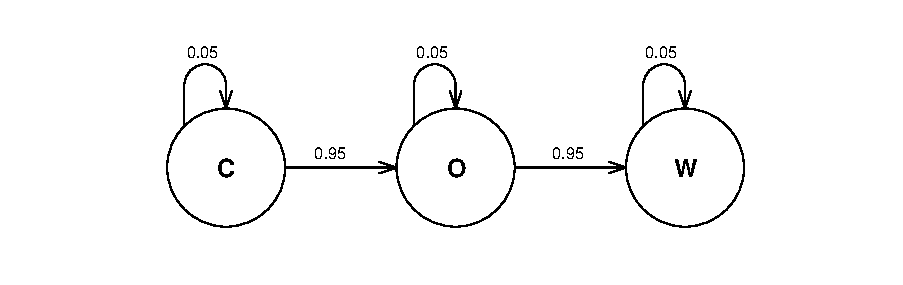
\includegraphics[scale=0.8]{billeder/simpleMarkov}
\caption{Markov model for the word "COW"}
\label{fig:simpleMarkov}
\end{figure}
		
In this model there is 0\% chance of moving from state "C" to "W". It is only possible to go to the same state, or change to the next in the letter series. This kind of model is called a Left-to-right model. This model is often used in this kind off application, but for other applications a other model where it is possible to jump between many states could be relevant. The states transaction is often given in a transaction matrix: 
\begin{equation}
	A_{n,n-1} = 
	\begin{bmatrix}
  	0.05 & 0.95 & 0 \\
  	0 & 0.05 & 0.95	\\
  	0 & 0 & 	1
 	\end{bmatrix}
 	\label{eq:Amat}
\end{equation}

In equation \ref{eq:Amat} the transition matrix is shown for the word "COW" illustrated by the transition graph in figure \ref{fig:simpleMarkov}. The matrix is an $M\times M$ matrix, where $M$ is the number of states. Each row and column is symbolizing the states, and the cells contains the transition probability from a row element to a column element.


\subsubsection{Hidden Markov Model}
A hidden Markov model is a Markov model in which the system being modelled is assumed to be a Markov process with unobserved states, also known as hidden states. It also have a set of desired output states. Like for the normal Markov model there is a transition between the hidden states given by a transition matrix $A$. For each hidden state there is also a probability of a given output state this is called the emission probability.

\begin{figure}[H]
\centering
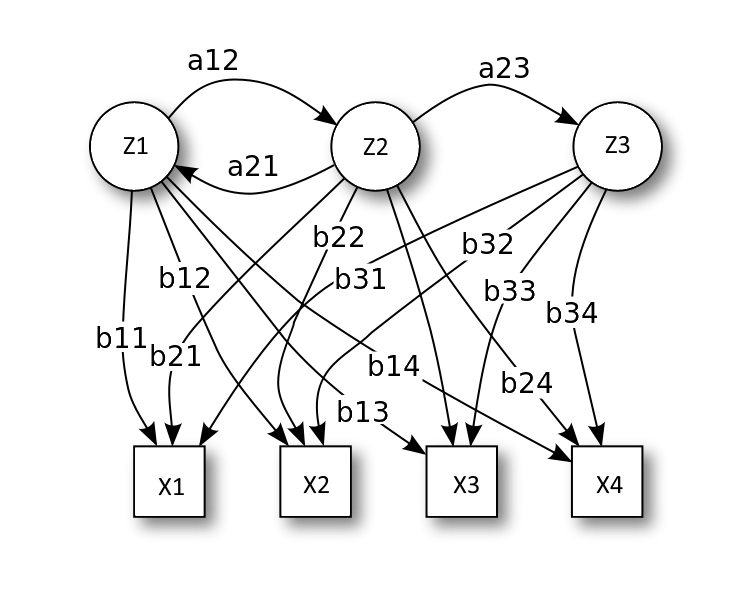
\includegraphics[scale=0.5]{billeder/HiddenMarkovModel}
\caption{Hidden Markov Model}
\label{fig:HiddenMarkov}
\end{figure}

This is illustrated on figure \ref{fig:HiddenMarkov}, where x is the known output states. The z is the hidden input states and a is the transaction parameters and b is the emission parameters. the probability for a given hidden sequence and output can be described as: 
\begin{equation}
 P(x_1, ..., x_n, z_1, ..., z_n) = P(z_1) \prod\limits_{n=2}^N{P(z_n| z_{n-1})} 
\prod\limits_{n=1}^N{P(z_n| z_n)}
\end{equation}
 
For many applications we do not know the hidden state of the data, but only the desired output state. It is therefore desired to make a training session that finds the optimal hidden states, and transition and emission parameters that gives us the best fit to the desired output states. 

